\chapter{Virtualización}

\section{Qué es la virtualización}

La virtualización es la creación de una versión virtual basada en software de algo, en lugar de una física. Se puede aplicar a sistemas operativos, almacenamiento, servidores, aplicaciones, redes… y es una manera de reducir gastos, aumentar eficiencia y agilidad en las empresas.  

\subsection{Tipos de virtualización}

Estos son los 4 tipos de virtualización más habituales.
\subsubsection{Virtualización de servidores}

La virtualización en servidores ayuda a evitar ineficiencias ya que permite ejecutar varios sistemas operativos en una máquina física como máquinas virtuales, con acceso a los recursos de todos. 
También permite generar un cluster de servidores en un único recurso para así mejorar mucho más la eficiencia y la reducción de costes. También permite el aumento de rendimiento de las aplicaciones, la disponibilidad al aumentar la velocidad en la carga de trabajo.

\subsubsection{Virtualización de escritorios}

La implementación de escritorios virtualizados permite ofrecer a las sucursales o empleados externos… de forma rápida y sencilla un entorno de trabajo y una reducción de la inversión a la hora de gestionar cambios en estos. 

\subsubsection{Virtualización de red}

Se trata de reproducir una red completa física mediante software, para poder ejecutar los mismo servicios que una red convencional y dispositivos. Cuentan con las misma características y garantías que las redes físicas con las ventajas que nos ofrece la virtualización más la liberación del hardware.

\subsubsection{Almacenamiento definido por software}

La virtualización del almacenamiento permite prescindir de  los discos de los servidores, los combina en depósitos de almacenamiento de alto rendimiento y los distribuye como software. Este nuevo modelo es permite aumentar la eficiencia en el guardado de datos.
\pagebreak  

\subsection{Ventajas de la virtualización}

Como se ha podido apreciar en los tipos de virtualización, esta conlleva una mejora considerable tanto en el rendimiento, agilidad, flexibilidad, escalabilidad… Como en una reducción de costes considerables tanto en tiempo como monetarios y una simplificación en la gestión de la infraestructura.

\begin{itemize}
\item Reduce los costes de capital y los gastos operativos.
\item Minimiza o elimina los tiempos de inactividad.
\item Aumenta la productividad, la eficiencia, la agilidad y la capacidad de respuesta.
\item Implementa aplicaciones y recursos con más rapidez.
\item Garantiza la continuidad del negocio y la recuperación ante desastres.
\item Simplifica la gestión del centro de datos. 
\end{itemize}

\section{Qué es Docker}

La idea detrás de Docker es crear contenedores ligeros y portables para las aplicaciones software que puedan ejecutarse en cualquier máquina con Docker instalado,
independientemente del sistema operativo que la máquina tenga por debajo, facilitando así también los despliegues.

De una manera más sencilla Docker los que nos proporciona es la opción de poder meter en pequeños contenedores todo aquello que nuestra aplicación necesite y poder desplegarla en cualquier maquina que tenga instalado Docker sin preocuparnos de nada más. 

Se podría decir que son pequeñas “máquinas virtuales” pero muchos más ligeras ya que utilizan el sistema operativo de donde se ejecuta y el contenido relevante para ejecutar la aplicación está dentro de los contenedores.
\newline 

Docker es:

\begin{itemize}
\item Open-Source para la gestión de "virtualización de contenedores"
\item Aísla múltiples sistemas de archivos en el interior del mismo host
\begin{itemize}
\item Las instancias se llaman Contenedores
\item Te dan la ilusión de estar dentro de una máquina virtual
\end{itemize}
\item Piensa en entornos de ejecución o "sandboxes"
\item No hay necesidad de un hypervisor (rápido de ejecutar)
\item Requiere x64 y Linux kernel 3.8+
\end{itemize}
\pagebreak 
Docker no es:

\begin{itemize}
\item Un lenguaje de programación
\item Un sistema operativo
\item Una máquina virtual
\item Una imagen en el concepto tradicional de la máquina virtual basada en hipervisor
\end{itemize}

\section{Máquinas Virtuales vs Docker}

Las máquinas virtuales, incluyen toda la aplicación, los binarios y librerías necesarias, y todo un sistema operativo cosa que hace que que ocupen mucho espacio, el tiempo de ejecución sea lento, la necesidad de un Hipervisor para su utilización.

Por lo contrario Docker container incluyen la aplicación y todas sus dependencias pero comparten el núcleo con otros contenedores, funcionando como procesos aislados en el sistema de ficheros del sistema operativo. Docker container no están vinculados a ninguna infraestructura específica: se ejecutan en cualquier ordenador, en cualquier infraestructura, y en cualquier cloud.

\begin{figure}[htb]
\begin{center}
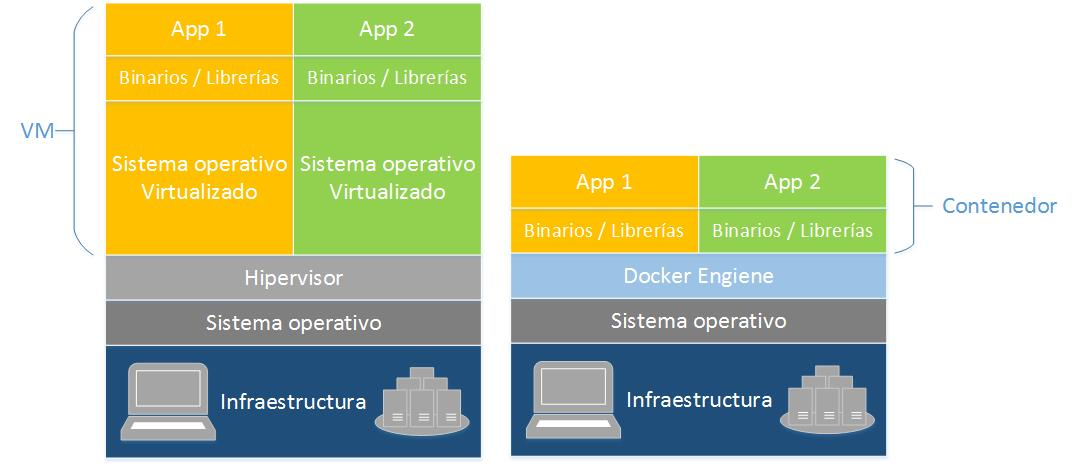
\includegraphics[width=1\textwidth]{./setup/VrvsDocker}
\caption{Comparativa de máquina virtual y Docker}
\label{F:VrvsDocker}
\end{center}
\end{figure}

En la imagen se puede apreciar la diferencias comentadas anteriormente, mientras la primera columna sería la virtualización de 3 aplicaciones se puede ver que hay la capa intermedia del Hipervisor el cual nos permite ejecutar los sistemas operativos virtualizados, todos los binarios y librerías que requieren cada aplicación y finalmente la aplicación. 
En la segunda columna tenemos la contenerización de 3 aplicaciones, podemos observar que no hace falta un hipervisor ya que utilizan el sistema operativo de la infraestructura donde se ejecuta, pero si son necesarios los binarios y las librerías.
A simple vista se puede apreciar que si eliminamos el sistema operativo la infraestructura completa se hace más liviana y rápida de ejecutar.

\section{Porque Docker?}

Por lo motivos listados en el apartados anteriores se decidió en utilizar Docker para realizar el despliegue de las aplicaciones, ya que se necesita de una tecnología la cual pueda ser almacenada en dispositivos con una memoria reducida en este caso docker la cumple. 

Su rapidez a la hora de levantar el servicio, en el mundo de IoT el tiempo es un bien preciado y los sistemas se pueden apagar y encender constantemente para evitar gastos de energía innecesarios.

La facilidad para poder desplegar los servicios, con Docker desplegar servicios es muy sencillo solo requiere tenerlo instalado y ejecutar el contenedor para que el servicio esté activo.

La sencillez a la hora de mantener el sistema, si hay que hacer actualizaciones o controles de una pequeña parte del servicio solo habria que cambiar o actualizar ese contenedor no todo el sistema. Esto es un gran ahorro en recursos y tiempo. 

Por todo esto se piensa que Docker puede ser una buena tecnología para desplegar sistemas de Iot. También se tiene en cuenta que la utilización de una Raspberry 3 no es un aparato con unas capacidades limitadas como podría ser un sensor utilizado normalmente pero si que puede validar todas las funciones listadas anteriormente y servir como preámbulo para la utilización en el resto de despliegues.  

